%!TEX root = emnlp2016.tex

In this section, we present the Capsule model for detecting and
characterizing significant diplomatic events. We first provide the
intuition behind Capsule, and then formally specify the model. We also
explain how to use Capsule to explore a corpus and how to learn the
posterior distribution of the latent variables.

\begin{figure}
\centering
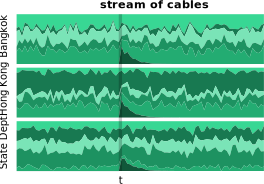
\includegraphics[width=\linewidth]{fig/cartoon.pdf}
\caption{Cartoon intuition. The $y$-axis represents the stacked
  proportions of cables about various topics, while the $x$-axis
  represents time. The Bangkok embassy, Honk Kong embassy, and
  U.S. State Department all have typical diplomatic business, about
  which they usually send cables. When an event occurs during time
  interval $t$, the cables alter to cover the event before returning
  to ``business as usual.'' Capsule discovers the embassies' typical
  concerns, as well as the timing and content of events.}
\label{fig:cartoon}
\end{figure}

Consider an entity like the Bangkok embassy, as illustrated in
figure~\ref{fig:cartoon}. We can imagine that this entity sends a
stream of diplomatic cables over time---some to the U.S. State
Department, others to other American embassies, such as the one in
Hong Kong. Embassies usually write cables that describe typical
diplomatic business. For example, the Bangkok embassy might write
about topics regarding southeast Asia more generally. We can think of
a topic as being a probability distribution over vocabulary terms.

Now imagine that an event, such as the capture of Saigon during the
Vietnam war, occurs during a particular time interval $t$. We cannot
directly observe the occurrence of this event, but we can observe the
stream of cables and the event's impact on it. When the event occurs,
multiple entities deviate from their usual topics of discussion
simultaneously, before returning to their usual behavior, as depicted
in figure~\ref{fig:cartoon}. For example, the day after the capture of
Saigon, the majority of the diplomatic cables written by the Bangkok
embassy and several other entities were about Vietnam war refugees. If
we think of the event as another probability distribution over
vocabulary terms, then each entity's stream of cables reflects its
typical concerns, as well as any significant events.


% \parhead{Background: Topic Models.} Capsule builds on topic models.  Topic models are algorithms for discovering the main themes in a large collection of documents; each document can then be summarized in terms of the global themes.  More formally, a topic $k$ is a probability distribution over the set of vocabulary words.  Each document $d$ is represented as a distribution over topics $\theta_d$.  Thus we can imagine that when we generate a document, we first pick which topics are relevant (and in what proportions).  Under the LDA topic model~\cite{Blei:2003}, we know the number of words in each document.  Then, for each word, we select a single topic from this distribution over topics, and finally select a vocabulary term from the corresponding topic's distribution over the vocabulary.  Alternatively, we can cast topic modeling as factorization, such as in Poisson factorization~\cite{Gopalan:2014b}, and draw a word count for each term in the vocabulary.

% Topic models are often applied to provide a structure for an
% otherwise unstructured collection of documents.  Documents, however,
% are often accompanied by metadata, such as the date written or
% author attribution; this information is not exploited by traditional
% topic models.  The Capsule model uses both author and date
% information to identify and characterize events that influence the
% content of the collection.

\subsection{Model Specification}
\label{sec:model_spec}

We now define the Capsule model. Our data come from \emph{entities}
(e.g., embassies) who send \emph{messages} (e.g., diplomatic cables)
over \emph{time}; specifically, we observe the number of times
$n_{dv}$ that each vocabulary term $v$ occurs in each message
$d$. Each message is associated with an author entity $a_d$ and a time
interval $t_d$ within which that message was sent.

We model each message with a bank of Poisson distributions---one for
each vocabulary term:
\begin{align}
  n_{dv} \sim \textrm{Poisson}\left(\lambda_{dv}\right).
\end{align}
The rate $\lambda_{dv}$ blends the different influences on message
content. Specifically, it blends three types of \emph{topics},
intended to capture ``business-as-usual'' discussion and content
related to significant events.

We operationalize each topic as a specialized probability distribution
over vocabulary terms (the set of unique words in the corpus of
messages), as is common in topic
models~\cite{Blei:2003,canny2004gap,Gopalan:2014b}---i.e., each term
is associated with each topic, but with a different probability.

\begin{table}
\centering
\small
\begin{tabular}{cc}
\toprule
Topic Type & Top Terms \\
\midrule
General & visit, hotel, schedule, arrival \\
Entity & soviet, moscow, ussr, agreement \\
Event & saigon, evacuation, vietnam, help \\
\bottomrule
\end{tabular}
\caption{The highest-probability vocabulary terms for examples of the
  three types of topics (general, entity, and event). These examples
  come from the analysis that we describe section~\ref{sec:eval}.}
\label{tab:3topics}
\end{table}

Each message blends 1) general topics $\mathbold{\beta}_1, \ldots,
\mathbold{\beta}_K$ about diplomacy (e.g., terms about diplomats,
terms about communication), 2) an entity topic $\mathbold{\eta}_{a_d}$
specific to the author of that message (e.g., terms about
Asia),\footnote{The entity-specific topics play a similar role to the
  background topics first introduced by Paul and
  Dredze~\shortcite{paul2012model}.} and 3) event topics
$\mathbold{\gamma}_1, \ldots, \mathbold{\gamma}_T$ that are specific
to the events in recent time intervals (e.g., terms about a coup,
terms about the death of a dignitary).

Examples of these three types of topics are in
table~\ref{tab:3topics}. The general topic relates to planning travel,
the entity topic captures words related to the U.S.S.R., and the event
topic captures words related to the evacuation of Saigon toward the
end of the Vietnam War.

The messages share the three types of topics in different ways: all
messages share the general topics, messages written by a single entity
share an entity topic, and messages in the same time interval use the
event topics in similar ways. Each message blends its corresponding
topics with a set of message-specific strengths. As a result, each
message captures a different mix of general diplomacy discussion,
entity-specific terms, and recent events. Specifically, the Poisson
rate for vocabulary term $v$ in message $d$ is
\begin{align}
  \lambda_{dv} &= \sum_{k=1}^K \theta_{dk} \beta_{kv}  + \zeta_d
  \eta_{a_dv} + {}\notag \\
  &\quad
  \sum_{t=1}^T f(t_d, t)\, \epsilon_{dt} \gamma_{tv},
\label{eq:poisrate}
\end{align}
where $\theta_{dk}$ is message $d$'s strength for general topic $k$,
$\zeta_{d}$ is message $d$'s strength for $a_d$'s entity topic, and
$\epsilon_{dt}$ is message $d$'s strength for event topic $t$. The
function $f(\cdot)$ ensures that the events influences decay over
time. We find that an exponential decay function, as in
equation~\ref{eq:f}, works well in practice.

We place hierarchical gamma priors over the message-specific
strengths, introducing entity-specific strengths $\mathbold{\phi}_1,
\ldots, \mathbold{\phi}_A$ and $\xi_1, \ldots, \xi_A$ that allow
different entities to focus on different topics and event strengths
$\psi_1, \ldots, \psi_T$ that allow different time intervals to be
more or less ``eventful.'' We place Dirichlet priors over the
topics. The graphical model is in figure~\ref{fig:graphicalmodel} and
the generative process is in figure~\ref{fig:generative-model}.

% NEED TO REMAKE THIS to use A rathre than N and n rather than w
\begin{figure}[bt]
\centering
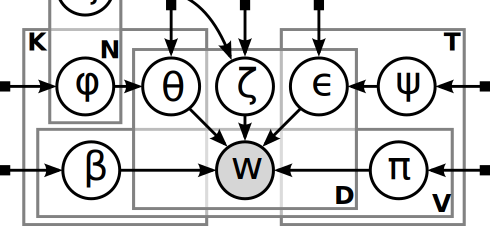
\includegraphics[width=0.5\linewidth]{fig/graphicalmodel.pdf}
\caption{Graphical model for Capsule. Observed word counts depend on
  general topics $\mathbold{\beta}_1, \ldots, \mathbold{\beta}_K$,
  entity topics $\mathbold{\eta}_1, \ldots, \mathbold{\eta}_A$, and
  event topics $\mathbold{\gamma}_1, \ldots, \mathbold{\gamma}_T$, as
  well as message-specific strengths $\mathbold{\theta}_d$, $\zeta_d$,
  and $\mathbold{\epsilon}_d$.  Variables $\mathbold{\phi}_1, \ldots,
  \mathbold{\phi}_A$ and $\xi_1, \ldots, \xi_A$ represent
  entity-specific strengths, while $\psi_1, \ldots, \psi_T$ allow time
  intervals to be more or less ``eventful.'' Black squares denote
  hyperparameters (unlabeled for visual simplicity).}
\label{fig:graphicalmodel}
\end{figure}

\begin{figure}[!ht]
\begin{mdframed}[userdefinedwidth=3.0in,align=center]
\small
\begin{itemize}[leftmargin=*]
\item for each time interval $t = 1, \ldots, T$,
	\begin{itemize}[leftmargin=*]
	\item draw event topic\\ $\mathbold{\gamma}_t \sim
          \textrm{Dirichlet}_V(\alpha, \ldots, \alpha)$
	\item draw event strength \\$\psi_{t} \sim \textrm{Gamma}\,(s, r)$
	\end{itemize}
\item for each entity $a = 1, \ldots, A$,
	\begin{itemize}[leftmargin=*]
	\item draw entity topic \\$\mathbold{\eta}_a \sim
          \textrm{Dirichlet}_V (\alpha, \ldots, \alpha)$
	\item draw entity-specific strength \\$\xi_{a} \sim \textrm{Gamma}\,(s, r)$
	\end{itemize}
\item for $k= 1, \ldots, K$,
	\begin{itemize}[leftmargin=*]
	\item draw general topic\\ $\mathbold{\beta}_k \sim
          \textrm{Dirichlet}_V (\alpha, \ldots, \alpha)$
	\item for each entity $a=1, \ldots, A$,
		\begin{itemize}[leftmargin=*]
		\item draw entity-specific strength \\$\phi_{ak} \sim \textrm{Gamma}\,(s, r)$
		\end{itemize}
	\end{itemize}
\item for each message $d= 1, \ldots, D$, sent at time interval $t_d$
  by author entity $a_d$,
	\begin{itemize}[leftmargin=*]
	\item draw local entity concern \\$\zeta_{d} \sim \mbox{Gamma}(s_\zeta, \xi_{a_d})$
	\item for each topic $k=$~1:$K$,
		\begin{itemize}[leftmargin=*]
			\item draw local entity concern \\$\theta_{d,k} \sim \mbox{Gamma}(s_\theta, \phi_{a_d,k})$
		\end{itemize}
	\item for each time $t=$~1:$T$,
		\begin{itemize}[leftmargin=*]
			\item draw local interval relevancy \\$\epsilon_{d,t} \sim \mbox{Gamma}(s_\epsilon, \psi_{t})$
		\end{itemize}
	\item for each vocabulary term $v=$~1:$V$,
		\begin{itemize}[leftmargin=*]
			\item set $\lambda_{d,v} = \theta_d^\top\beta_v  + \zeta_d \eta_{a_d} +$\\$ \sum_{t=1}^T f(i_d, t) \epsilon_{d,t} \gamma_{t,v}$
			\item draw word counts \\$w_{d,v} \sim \mbox{Poisson}\left(\lambda_{d,v}\right)$
		\end{itemize}
	\end{itemize}
\end{itemize}
\end{mdframed}
\caption{The generative process for Capsule.}
\label{fig:generative-model}
\end{figure}

Given a corpus of messages, learning the posterior distribution of the
latent variables uncovers the three types of topics, the message- and
entity-specific strengths, and the event strengths. In section~\ref{},
we explain how an analyst can use the event strengths as a filter that
isolates potentially significant messages.

% HMW: I moved the paragraph about Hawkes processes to related work.

\subsection{Learning the Posterior Distribution}


In order to use the Capsule model to explore the observed documents, we must compute the posterior distribution.  Conditional on the observed word counts $w$, our goal is to compute the posterior values of the hidden parameters---general topics $\beta$, entity topics $\eta$, event topics $\gamma$, entity concerns $\phi$ (for general topics) and $\xi$ (for their own topic), overall event strengths $\psi$, and document-specific strengths for general topics $\theta$, entity topics $\zeta$, and event topics $\epsilon$.

As for many Bayesian models, the exact posterior for Capsule is not tractable to compute; approximating it is our central statistical and computational problem.  We develop an approximate inference algorithm for Capsule based on variational methods~\cite{Jordan:1999},\footnote{Source code is available at \url{https://github.com/ajbc/capsule}.} which is detailed in \Cref{sec:inference}.\footnote{Appendices are located in the supplemental materials document.} This algorithm produces a fitted variational distribution which can then be used as a proxy for the true posterior, allowing us to explore a collection of documents with Capsule.


\parhead{Detecting and characterizing events.}
Once we estimate the posterior distribution of the Capsule parameters, described in the following section, we can use the expectations of the latent parameters to explore the original data.  To detect events, we consider the proportion of the document about event $j$, and take a weighted average of these proportions:
\begin{equation*}
m_j = \frac{1}{\sum_{d} f(i_d, j)} \sum_{d}\frac{\varepsilon_{d,j}}{\zeta_d + \sum_{t} \varepsilon_{d,t} + \sum_{k} \E[\theta_{d,k}] },
\label{eq:eventness}
\end{equation*}
where $\varepsilon_{d,t} = f(i_d, t) \E[\epsilon_{d,t}]$.
This measure of ``eventness'' provides an estimate of the proportion of words that are related to a real-world event in that interval.  Figure~\ref{fig:cables_events} shows events detected with this metric.

Given an identified event, we can characterize it in terms of its top terms under $\gamma$, but we can also use weighted event relevancy parameters $\varepsilon_{d,t}$ to sort documents; \Cref{sec:eval} explores relevant documents for events found in the National Archive diplomatic cables data.
In addition to detecting and characterizing events, Capsule can be used to explore entity concerns and the general themes in a given collection.

To make Capsule more accessible, we developed an open source tool for visualizing its results.\footnote{Source code: \url{https://github.com/ajbc/capsule-viz}; demo: \url{http://www.princeton.edu/~achaney/capsule/}.}  Our tool creates a navigator of the documents and latent parameters, allowing users to explore events, entities, topics, and the original documents.  Figure~\ref{fig:viz} shows several screenshots of this browsing interface.

\begin{figure}
\centering
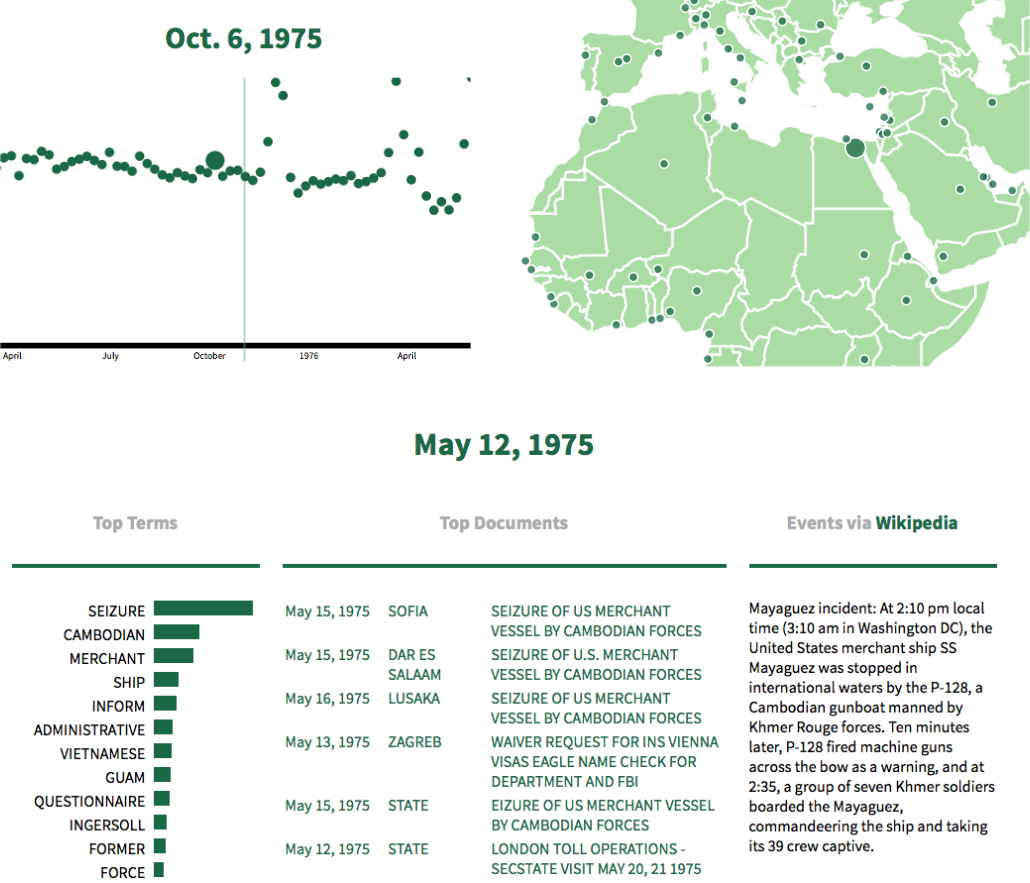
\includegraphics[width=\linewidth]{fig/viz.png}
\caption{Screenshots of Capsule visualization of US State Department cables.  Top-left: events over time (similar to \Cref{fig:cables_events}).  Right-top: entities shown on a map.  Bottom: time interval summary, including top terms, relevant documents, and text scraped from Wikipedia.}
\label{fig:viz}
\end{figure}
